\subsection{Impact of lattice calculations of  $x$-space PDFs}
\label{sec:projectionsxspace}

In the previous section, we studied the impact of
lattice-QCD calculations of PDF moments. 
%
We now perform an exploration of the
potential constraints that future lattice QCD calculations
of $x$-space PDFs can provide on global analyses.
%
We focus on the isotriplet
combination $x u-x d$ (and $x\Delta u - x\Delta d$
in the polarized case), the quark combination 
on which initial studies have been focused, as
it is the simplest to calculate, owing to the lack of disconnected
diagrams and the absence of mixing with other quark flavors or with gluons.


Following the same Bayesian reweighting procedure employed for PDF moments
in Sec.~\ref{sec:projections:rw},
we have generated pseudo-data for the isotriplet
combinations
\be
\label{eq:isotriplet_unpol}
u(x_i,Q^2)-d(x_i,Q^2) \, \quad\text{and} \, \quad
\bar{u}(x_i,Q^2)-\bar{d}(x_i,Q^2) \, , \quad i=1,\ldots,N_x \, ,
\ee
for the unpolarized case, and for
\be
\label{eq:isotriplet_pol}
\Delta u(x_i,Q^2)-\Delta d(x_i,Q^2) \, \quad\text{and} \, \quad
\Delta\bar{u}(x_i,Q^2)-\Delta\bar{d}(x_i,Q^2) \, , \quad i=1,\ldots,N_x \, ,
\ee
for the polarized case, with $N_x$ being the number of points
in $x$-space that are being sampled.
%
We take $Q^2=4\text{ GeV}^2$, consistent with our choices for the exercise 
performed in Secs.~\ref{sec:projections:rw}--\ref{sec:hessianprofiling}.

We consider three scenarios, denoted by Scenarios D, E, and F,
for the total uncertainty $\delta_L^{(i)}$
that will be assigned to
the lattice-QCD calculations of the specific quark
combinations listed in Eqs.~\eqref{eq:isotriplet_unpol}
and \eqref{eq:isotriplet_pol}.
%
Lattice-QCD computations are expected to have the smallest systematic 
uncertainties at large $x$, so we choose the $N_x=5$ points to be
\be
x_i = 0.70\, ,0.75,\, 0.80,\, 0.85, \, 0.90 \, .
\ee
%
For each scenario, we assume the same relative error for each value of 
$\{x_i\}$, and we neglect possible correlations between 
neighboring $x$-points.
%
We assume uncertainties of $\delta_{L}^{(i)}=12\%, 6\%$ and 3\% for scenarios
D, E, and F, respectively.
%
Note that we assume the same values of $\delta_{L}^{(i)}$ for the polarized
and unpolarized cases, as well as for both the quark
and antiquark isotriplet combinations Eqs.~\eqref{eq:isotriplet_unpol}
and \eqref{eq:isotriplet_pol}.

We summarize the results of this exercise in Fig.~\ref{fig:impactxspace}, 
where we plot the ratio of the PDF uncertainties in each Scenarios A, B and C 
(D, E and F) to the uncertainty of the original
NNPDF3.1 (NNPDFpol1.1) set.
%
We show the impact on the PDF uncertainties
in $\bar{u}$ and $\bar{d}$ at large-$x$ in the upper
plots, with the corresponding comparison for $\Delta\bar{u}$
and $\Delta\bar{d}$ in the lower plots.
%
We concentrate on the results for the individual quark flavors, even though 
the constraints are imposed on differences between flavors, as the former are 
of the more direct interest for phenomenology. 
%
From this comparison, we find that lattice-QCD calculations of the 
$x$-dependence of PDFs can significantly reduce the uncertainties for both 
unpolarized and polarized antiquarks in the large-$x$ region.
%
Taking into account that the PDF uncertainties on the large-$x$
antiquarks are rather large, and that they
enter a number of important Beyond the Standard Model (BSM) search channels
(such as for instance for production of new heavy gauge bosons $W'$ and $Z'$),
our analysis demonstrates that such calculations would have direct
phenomenological implications.
%
We note however that the curves in Fig.~\ref{fig:impactxspace}
fluctuate by a rather large amount.
%
This might be due to the fact that the uncertainties of the original PDFs
fluctuate, particularly at low scales.

%-------------------------------------------------------------------
\begin{figure}[!t]
\centering
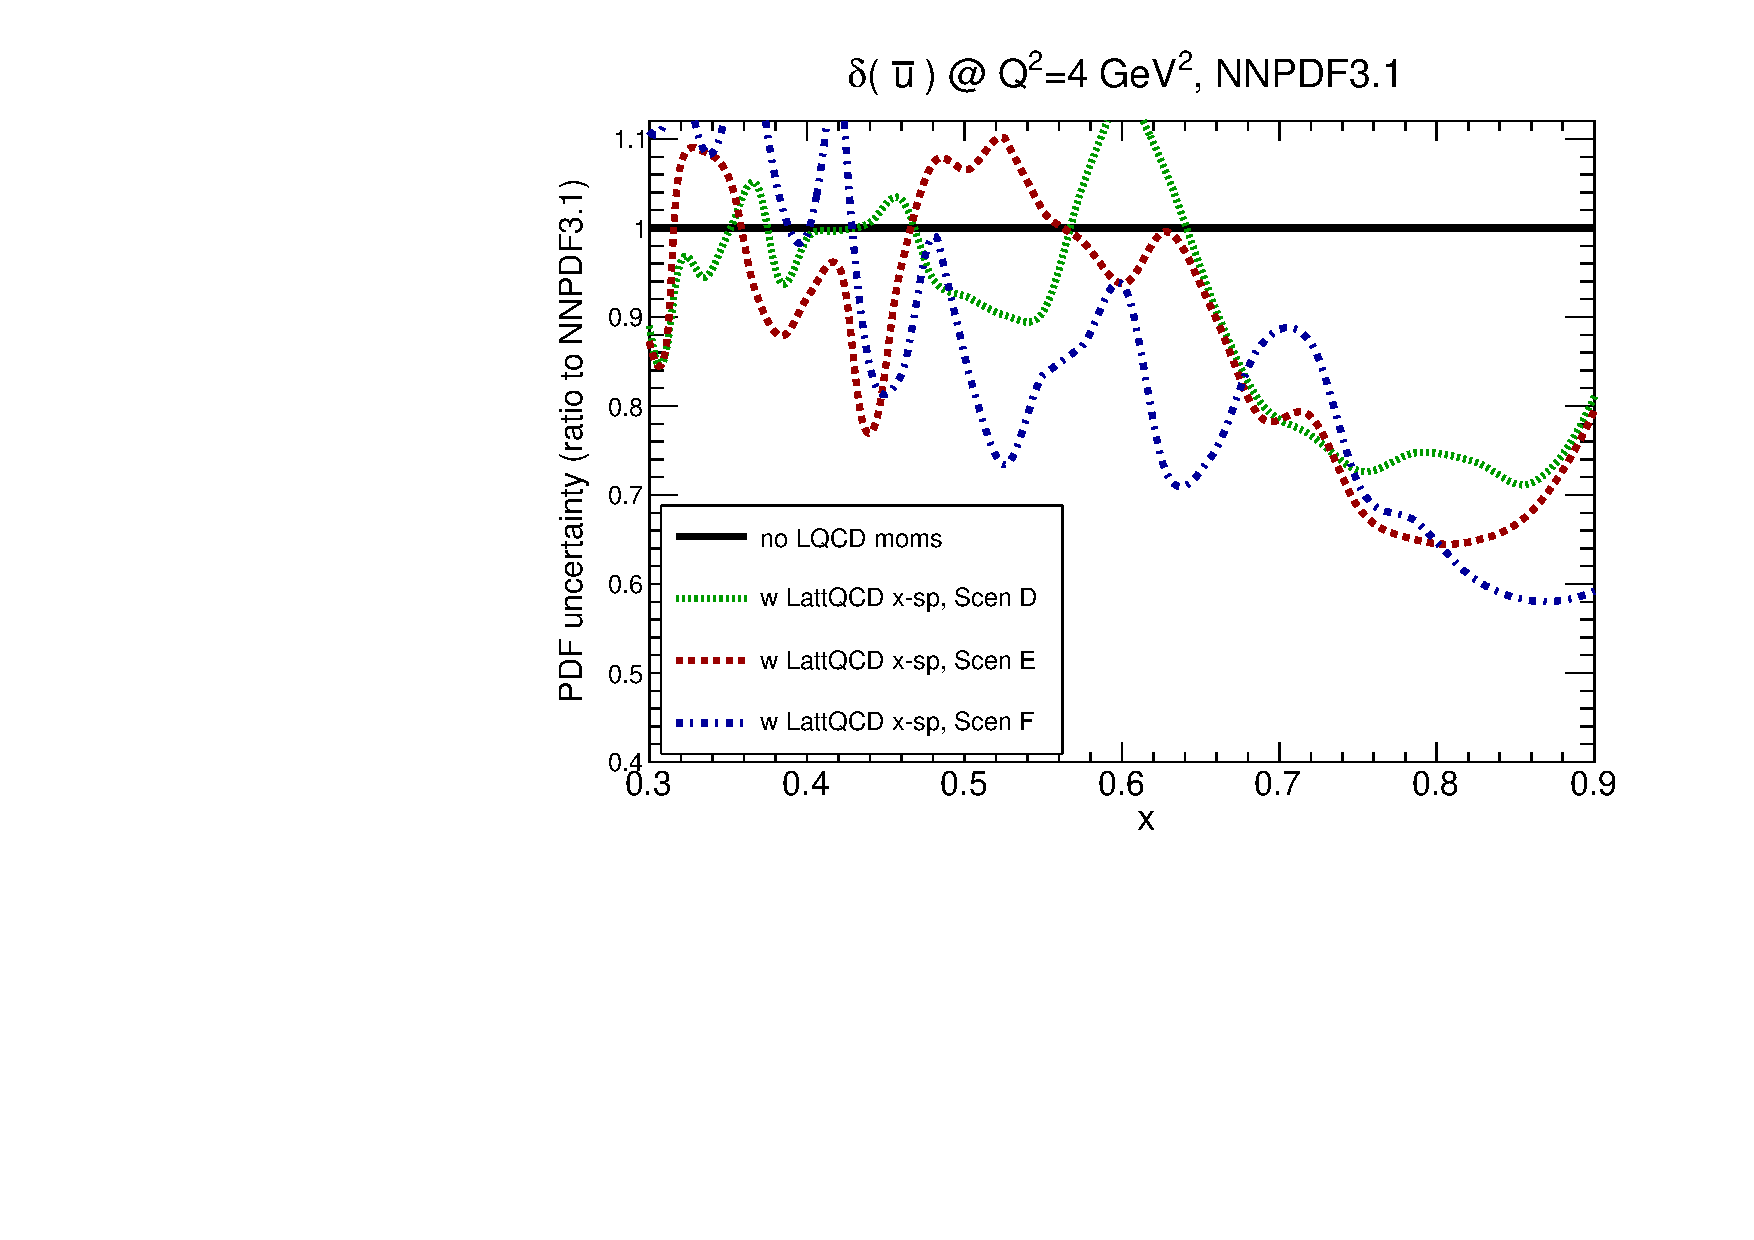
\includegraphics[scale=0.45]{plots/xubar-unpol-lattice-relerr-xdata-xspace.pdf}
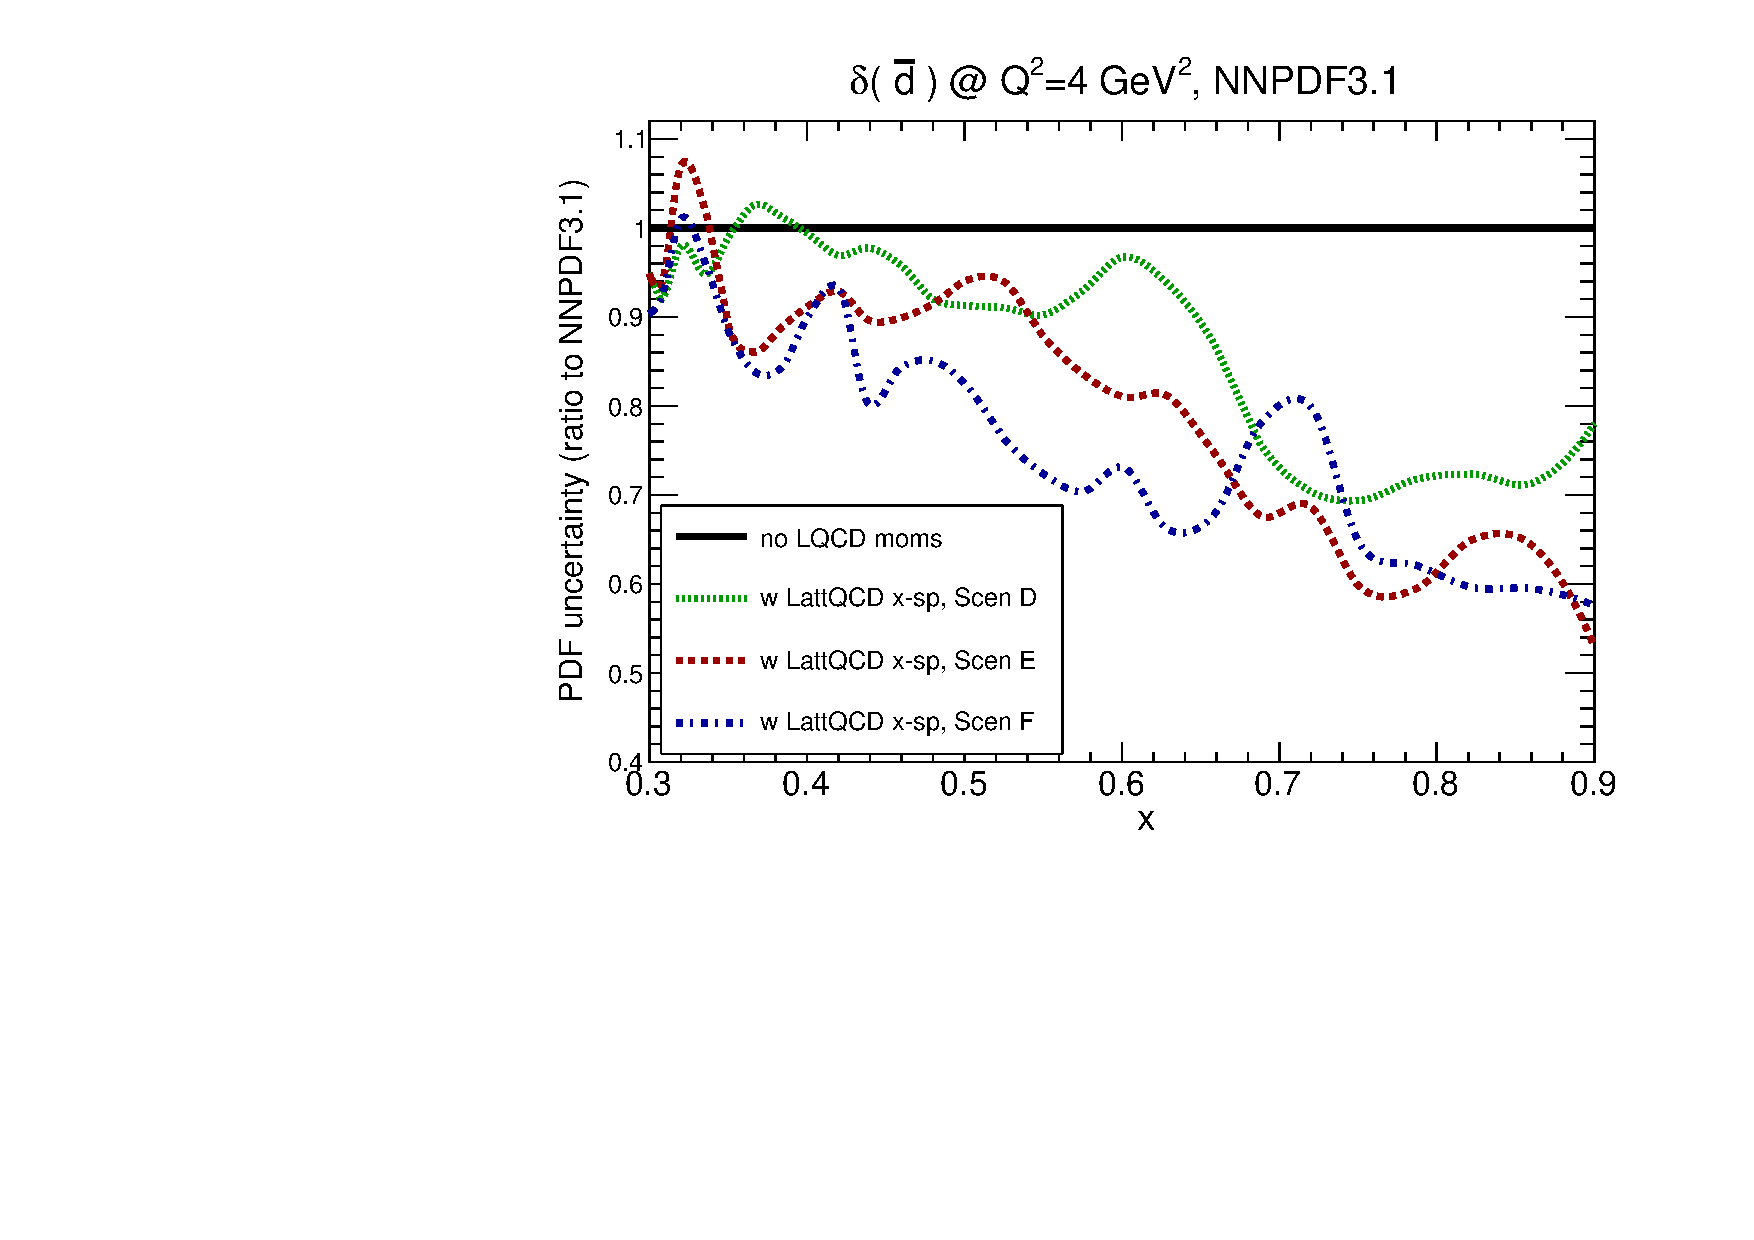
\includegraphics[scale=0.45]{plots/xdbar-unpol-lattice-relerr-xdata-xspace.pdf}
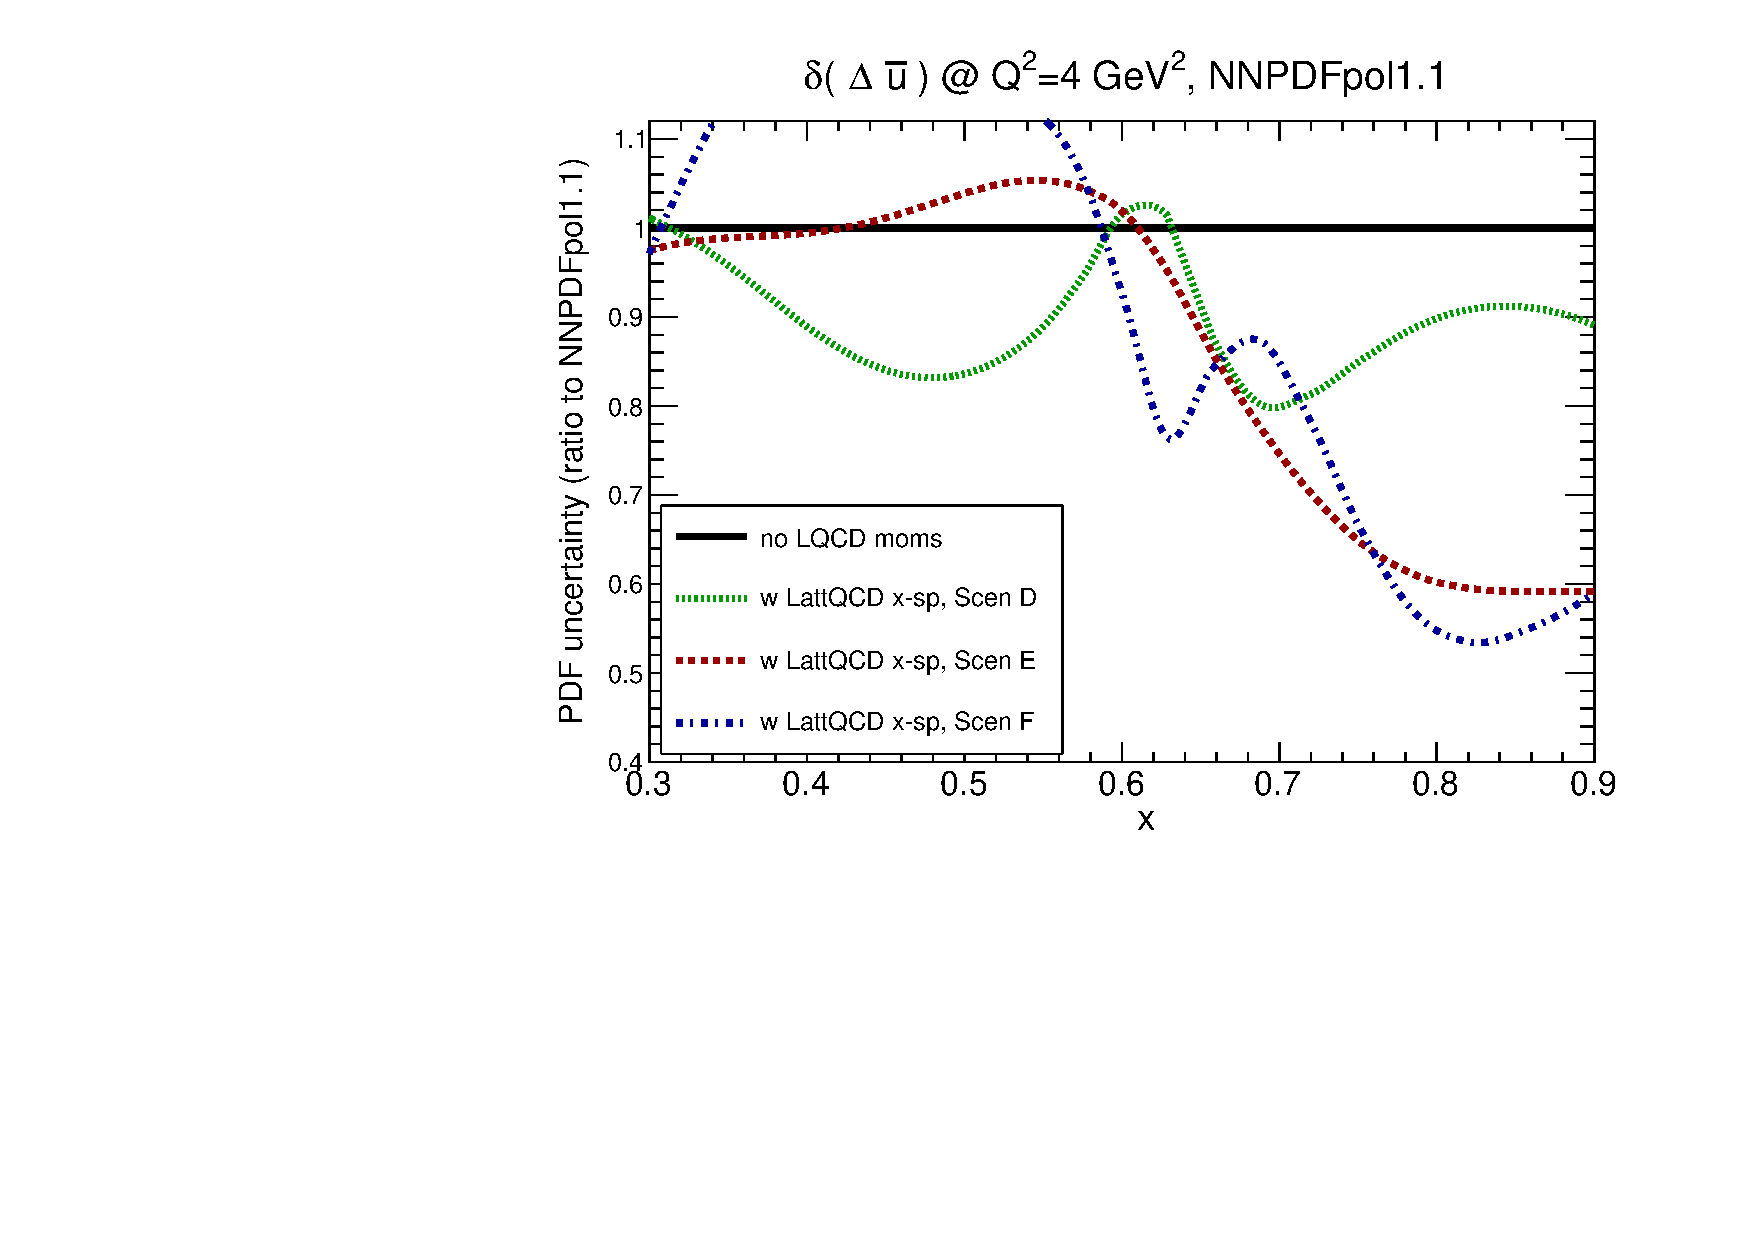
\includegraphics[scale=0.45]{plots/xubar-pol-lattice-relerr-xdata-xspace.pdf}
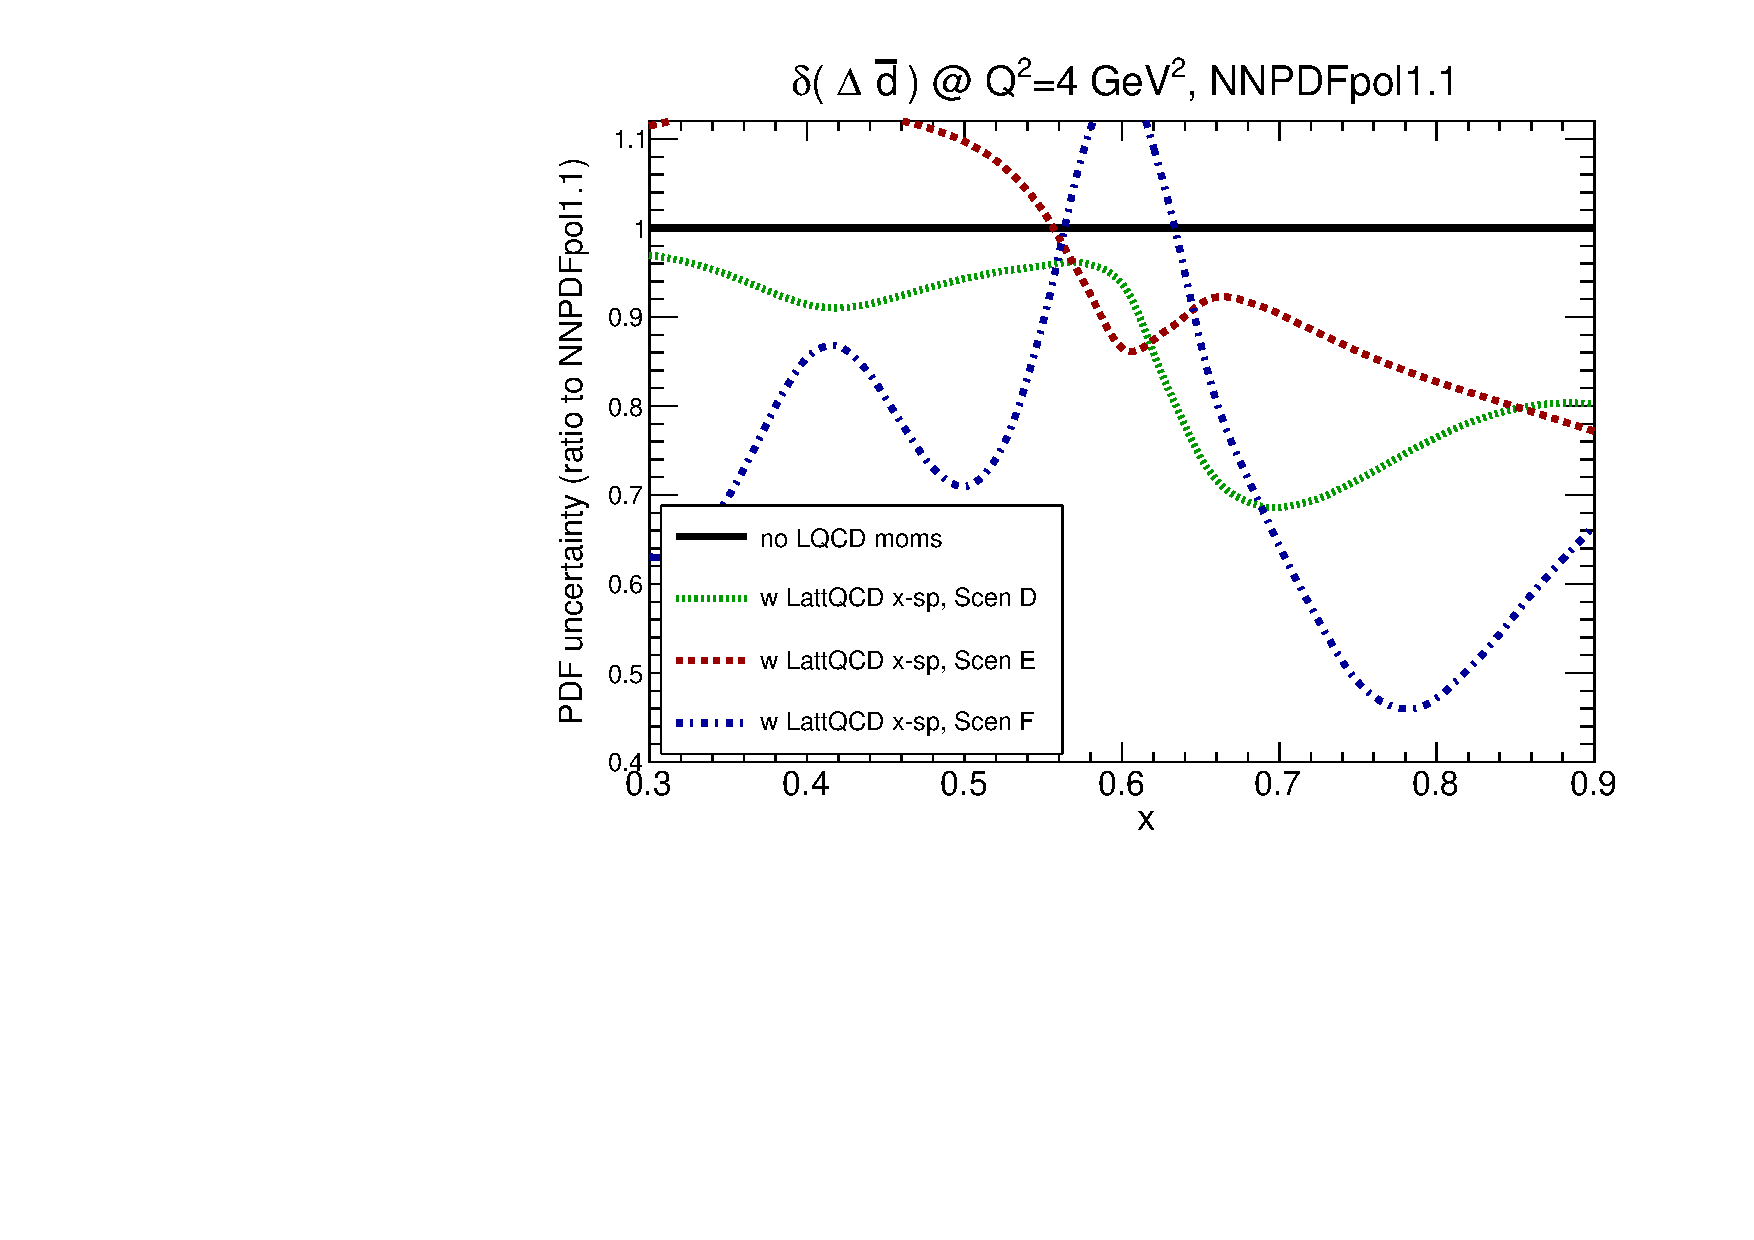
\includegraphics[scale=0.45]{plots/xdbar-pol-lattice-relerr-xdata-xspace.pdf}
\caption{\small The ratio of PDF uncertainties to the original
  NNPDF3.1 (NNPDFpol1.1) in the fits where lattice-QCD pseudo-data
  on $x$-space PDFs have been added to the global unpolarized
  (polarized) analysis.
  %
  Specifically, we show the impact on the PDF uncertainties
  in $\bar{u}$ and $\bar{d}$ at large-$x$ in the upper
  plots, with the corresponding comparison for $\Delta\bar{u}$
  and $\Delta\bar{d}$ in the lower plots.
}    
\label{fig:impactxspace}
\end{figure}
%---------------------------------------------------------------------

Fig.~\ref{fig:impactxspace} shows that
in the unpolarized case the large-$x$ PDF uncertainties could be reduced
to $60\%$ of their original value.
%
We also find that there are no large
differences between the three
scenarios,
probably because the constraint is on quark differences not on individual 
flavors, so there is freedom for $\bar u$ and $\bar d$ to vary in a correlated 
fashion while still satisfying the constraint. 
%
However, it does suggest 
that a direct lattice-QCD calculation
of $x \bar{u}-x \bar{d}$ does not need to reach uncertainties
at the few-percent level to influence global fits.
%
For the polarized PDFs, Fig.~\ref{fig:impactxspace} demonstrates that the
reduction in PDF uncertainties could be significantly more marked.
%
For instance, in the case of $\Delta \bar{d}$, at $x\simeq 0.8$
the resulting PDF uncertainty from Scenario~F is less than 50\%
of the original uncertainty.

In Table~\ref{tab:neffxspace} we indicate the effective number of replicas
$N_\text{eff}$, Eq.~\eqref{eq:effnrep}, remaining when
the lattice-QCD pseudo-data for Eqns.~\eqref{eq:isotriplet_unpol}
and~\eqref{eq:isotriplet_pol} are included in the global
unpolarized and polarized fits.
%
Here we find a marked decrease in $N_\text{rep}$
for the three scenarios,
in particular for the unpolarized case.
%
For example, in the most optimistic Scenario~F, only
64 effective replicas remain out of the
original sample of $N_\text{rep}=1000$ replicas.
%
See Table~\ref{tab:neff} for the corresponding
information at the level of PDF moments.
   
%------------------------------------------------------------------------------
\begin{table}[!t]
\centering
\footnotesize
\renewcommand{\arraystretch}{1.3} 
\begin{tabular}{lcc}
\toprule
&  NNPDF3.1  &  NNPDFpol1.1 \\
\midrule
$N_\text{rep}$ original   & 1000 & 100 \\
$N_\text{eff}$ Scenario D &  376 &  41 \\
$N_\text{eff}$ Scenario E &  173 &  35 \\
$N_\text{eff}$ Scenario F &  64  &  22 \\
\bottomrule
\end{tabular}
\caption{\small The effective number of replicas
  $N_\text{eff}$, Eq.~\eqref{eq:effnrep}, remaining when the pseudo-data
  on the lattice-QCD calculations
  of Eqns.~\eqref{eq:isotriplet_unpol}
  and~\eqref{eq:isotriplet_pol} 
  are included in the global
  unpolarized and polarized fits. 
  \label{tab:neffxspace}
  }
\end{table}
%-------------------------------------------------------------------------------

We emphasize that the results of this exercise must be interpreted
with some care.
%
First of all, the results depend sensitively on the specific values of
$\left\{ x_i \right\}$
that we have assumed for the lattice-QCD calculation,
and on the values
of the associated uncertainties $\delta_L^{(i)}$.
%
The quantitative results depend on the choice of input PDF set and would 
vary if, for example, the input set were the HERAPDF2.0 set used for the 
Hessian profiling exercise of Sec.~\ref{sec:hessianprofiling}.
%
Even with these caveats, our analysis makes clear that a direct
computation of the isotriplet combination $x u-x d$ on the lattice
has the potential to constrain the large-$x$ PDFs in
a more significant way than corresponding PDF moment calculations,
particularly in the unpolarized case.
%
Given the importance of antiquark PDFs in the large-$x$ region for LHC 
phenomenology (especially for a high-luminosity run), 
pursuing these calculations should be high on the list
of priorities for the lattice-QCD community.


